\section{Results}
% All this Sec.~will be 1/2 pages.


%The testing process began with a single worker (centralized \gls*{gan}) in order to determine the optimal layer architecture for the generator and discriminator. We initially conducted the testing using anomalous data, and then normal data was introduced later on.
\textcolor{blue}{We compared the performance of a centralized \gls*{gan} (i.e., a single worker) with our decentralized approach. For evaluation, we trained 3 separate auto-regression models for each data behaviour (normal, anomalous, mixed). Each \gls*{trtr} model is needed to calculate the corresponding \gls*{trts} for the \gls*{gan} getting tested. The auto-regression models are set-up to predict the last five time steps.
%
We use the \gls*{trtr} metric (Tab.~\ref{tab:trtr-main}) to verify the results when applied to synthetic data. In particular, we tested each \gls*{trtr} on 10 different synthetic data samples from each generator to calculate an average for the \gls*{trts} metric. Similarly, we trained an auto-regression model with synthetic data 10 different times to calculate an average for the \gls*{tstr} metric.}


\subsection{Centralized GAN Results}

We tested the model initially using fixed sequence widths of 64, 128, and 256 seconds. The results show a sequence width of 64 seconds being the better performer if we used the fixed sequence strategy width. After applying the dynamic window strategy, both visual inspection and the \gls*{trts} / \gls*{tstr} (see Tab.~\ref{tab:dynamic-window}) showed an improvement. This confirms that the dynamic window in fact improves the capabilities of the generator in contrast to using a fixed sequence width. \textcolor{blue}{\marginnote{RC22}Our dynamic window strategy, confirmed superior via visual inspection, notably outperformed the comparable yet non-decentralized TimeGAN model in both \gls*{trts} and \gls*{tstr} metrics (see Tab.~\ref{tab:dynamic-window}). This result reinforces the advantage of our method over related existing models.}

\begin{table}[t]
\centering
\caption{Dynamic window effect (anomalous behaviour)}\marginnote{\textcolor{blue}{RC22}}
\label{tab:dynamic-window}
%\resizebox{\columnwidth}{!}{%
\begin{tabular}{lcccccc}
\Xhline{1.5pt}
\multicolumn{1}{c}{\multirow{2}{*}{\sc{\begin{tabular}[c]{@{}c@{}}Sequence \\ Width\end{tabular}}}} &
  \multicolumn{3}{c}{\sc{TRTS}} &
  \multicolumn{3}{c}{\sc{TSTR}} \\
\multicolumn{1}{c}{} &
  \sc{R2} &
  \sc{MAE} &
  \sc{RMSE} &
  \sc{R2} & 
  \sc{MAE} &
  \sc{RMSE} \\ \Xhline{1pt}
64 s  & 0.375 & 0.089 & 0.203 & 0.609 & 0.055	& 0.160 \\ \hline
128 s & 0.352 & 0.084 & 0.206 & 0.599 & 0.054	& 0.165 \\ \hline
256 s & 0.153 & 0.177 & 0.236 & -1.84 & 0.215	& 0.284 \\\hline
Dynamic     & 0.550 & 0.070 & 0.171 & 0.621 & 0.051 & 0.162\\ \Xhline{1.6pt}
\textcolor{blue}{TimeGAN}     & \textcolor{blue}{0.471}	& \textcolor{blue}{0.073}	& \textcolor{blue}{0.187}	& \textcolor{blue}{0.604}	& \textcolor{blue}{0.057}	& \textcolor{blue}{0.162}\\ \Xhline{1.5pt}
\end{tabular}%
%}
\end{table}





%
The normalization we used in previous tests employed the first technique mentioned in Sec.~\ref{sec:data-pre-process}, where each feature is normalized based on the known capabilities of that specific feature. We then further tested the second technique, where the normalization occurs based on the limits of the workers. The \gls*{trts} / \gls*{tstr} results in Tab.~\ref{tab:normalize-result} showed that using the worker limits yields a significant improvement. We adapted the second technique to all upcoming tests.
\begin{table}[t]
\centering
\caption{Worker normalization effect (normal behaviour)}
\resizebox{\columnwidth}{!}{%
\begin{tabular}{lcccccc}
\Xhline{1.5pt}
\multicolumn{1}{c}{\multirow{2}{*}{\sc{Normalization}}} & \multicolumn{3}{c}{\sc{TRTS}} & \multicolumn{3}{c}{\sc{TSTR}} \\ 
\multicolumn{1}{c}{}    & \sc{R2}    & \sc{MAE}   & \sc{RMSE}  & \sc{R2}    & \sc{MAE}   & \sc{RMSE}  \\ \Xhline{1.2pt}
Fixed Limits  &  0.472	& 0.096	& 0.169	& 0.743	& 0.133	& 0.164 \\ \hline
Worker Limits &  0.724	& 0.041	& 0.128	& 0.901	& 0.028	& 0.070 \\ \Xhline{1.5pt}
\end{tabular}%
}

\label{tab:normalize-result}
\end{table}






\subsection{Decentralized GAN Results}
%
We set-up the network with one server and four workers. Workers \#1 and \#2 had anomalous data, while workers \#3 and \#4 had normal data.
As shown in Fig.~\ref{fig:decentralized_results}, the output sequence generated by the most forgiving strategy only contain behaviour belonging to workers \#1 and \#2 (Anomalous), while the least forgiving strategy produces a mix of classes from both workers. This output shows both normal and anomalous behaviour, which looks similar to the mixed data behaviour shown in Fig.~\ref{fig:scania-data}. This can also be corroborated by examining the worker contribution count, which tracks the number of times each worker was selected for generator training (see Fig.~\ref{fig:work-cont-decentralized}. The most forgiving strategy exhibits a strong bias towards workers \#1 and \#2, while the least forgiving strategy exhibits a more balanced distribution. This explains the difference in output observed in the generated sequences.

\begin{table}[t]

\centering
\caption{FL strategy effect (mixed behaviour)}
\resizebox{\columnwidth}{!}{%
\begin{tabular}{lcccccc}
\Xhline{1.5pt}
\multicolumn{1}{c}{\multirow{2}{*}{\sc{FL Strategy}}} & \multicolumn{3}{c}{\sc{TRTS}} & \multicolumn{3}{c}{\sc{TSTR}} \\ 
\multicolumn{1}{c}{}    & \sc{R2}    & \sc{MAE}   & \sc{RMSE}  & \sc{R2}    & \sc{MAE}   & \sc{RMSE}  \\ \Xhline{1.2pt}

Most Forgiving & 0.504 & 0.070 & 0.176 & 0.426 & 0.067 & 0.177 \\  \hline
Weighted Average & 0.348 & 0.090 & 0.201 & 0.522 & 0.071 & 0.170 \\ \hline
Least Forgiving & 0.525	& 0.076	& 0.172	& 0.588	& 0.055	& 0.158 \\
\Xhline{1.5pt}

\end{tabular}
}

\label{tab:decentralized-tstr}
\end{table}





The behaviour of the most forgiving strategy can be understood as follows; in this approach, the generator is updated based on the worker with the highest loss on the fake data produced by the generator. This leads to the generator creating fake data that closely resembles the data of the selected worker. In subsequent iterations, it is expected that the previously selected worker will have a higher loss on the fake images, as the generator is more specialized to their data. On the other hand, the rest of the workers are likely to have a lower loss, insuring a much less likelihood of being selected. As the training process continues, the generator is expected to converge on a small subset of workers, effectively ignoring the data of other workers as the distribution of generated data is very different from their local data distribution. 

We also implemented and tested two different forms of weighting for the averaging technique (\gls*{f2a}), one that favoured the most forgiving worker and another that favoured the least forgiving worker. We used the Softmax function to determine the contribution of each worker to the overall average model. In the next iteration, all workers used the newly averaged discriminator model. However, there was a noticeable output degradation as suggested by the \gls*{trts} / \gls*{tstr} results and the output sequence shown in Fig.~\ref{fig:decentralized_results}.
%
\def\layerfigwidth{0.8}
\def\layerfigheight{0.25}
\def\ydist{-3.7}
\begin{figure} [t]
    \centering
\begin{tikzpicture}[scale = 0.61]
\begin{axis} [every axis plot post/.append style={mark=none,smooth,-,line width = \plotlinewidth pt},
ylabel={Most Forgiving},
axis x line=bottom,
axis y line=left,
axis line style={-,line width = 1pt},
% ticks=none,
width=\layerfigwidth\textwidth,
height=\layerfigheight\textwidth,
xmax = 1000,
ymax=1.005
] 
    \addplot[fone] table [col sep=comma,header=true,x index=0,y index=1] {Data/most_forgiving.csv};
    \addplot[ftwo] table [col sep=comma,header=true,x index=0,y index=2] {Data/most_forgiving.csv};
    \addplot[fthree] table [col sep=comma,header=true,x index=0,y index=3] {Data/most_forgiving.csv};
    \addplot[ffour] table [col sep=comma,header=true,x index=0,y index=4] {Data/most_forgiving.csv};
    \addplot[ffive] table [col sep=comma,header=true,x index=0,y index=5] {Data/most_forgiving.csv};  
    \addplot[fsix] table [col sep=comma,header=true,x index=0,y index=6] {Data/most_forgiving.csv};
    \addplot[fseven] table [col sep=comma,header=true,x index=0,y index=7] {Data/most_forgiving.csv};
    \addplot[feight] table [col sep=comma,header=true,x index=0,y index=8] {Data/most_forgiving.csv};
\end{axis}


\begin{axis} [at={(0,\ydist cm)},every axis plot post/.append style={mark=none,smooth,-,line width = \plotlinewidth pt},
% xlabel={Time Step [s]},
ylabel={Weighted Average},
axis x line=bottom,
axis y line=left,
axis line style={-,line width = 1pt},
% ticks=none,
width=\layerfigwidth\textwidth,
height=\layerfigheight\textwidth,
xmax = 1000,
ymax=1.005
]
    \addplot[fone] table [col sep=comma,header=true,x index=0,y index=1] {Data/weighted_avg.csv};
    \addplot[ftwo] table [col sep=comma,header=true,x index=0,y index=2] {Data/weighted_avg.csv};
    \addplot[fthree] table [col sep=comma,header=true,x index=0,y index=3] {Data/weighted_avg.csv};
    \addplot[ffour] table [col sep=comma,header=true,x index=0,y index=4] {Data/weighted_avg.csv};
    \addplot[ffive] table [col sep=comma,header=true,x index=0,y index=5] {Data/weighted_avg.csv};  
    \addplot[fsix] table [col sep=comma,header=true,x index=0,y index=6] {Data/weighted_avg.csv};
    \addplot[fseven] table [col sep=comma,header=true,x index=0,y index=7] {Data/weighted_avg.csv};
    \addplot[feight] table [col sep=comma,header=true,x index=0,y index=8] {Data/weighted_avg.csv};
\end{axis}

\begin{axis} [at={(0,\ydist*2 cm)},every axis plot post/.append style={mark=none,smooth,-,line width = \plotlinewidth pt},
xlabel={Time Step [s]},
ylabel={Least Forgiving},
axis x line=bottom,
axis y line=left,
axis line style={-,line width = 1pt},
% ticks=none,
width=\layerfigwidth\textwidth,
height=\layerfigheight\textwidth,
xmax = 1000,
ymax=1.005,
legend columns=4,
legend style={at={(0.5,-0.5)},anchor=north,font=\large}
]
    \addplot[fone] table [col sep=comma,header=true,x index=0,y index=1] {Data/least_forgiving_2.csv};
    \addplot[ftwo] table [col sep=comma,header=true,x index=0,y index=2] {Data/least_forgiving_2.csv};
    \addplot[fthree] table [col sep=comma,header=true,x index=0,y index=3] {Data/least_forgiving_2.csv};
    \addplot[ffour] table [col sep=comma,header=true,x index=0,y index=4] {Data/least_forgiving_2.csv};
    \addplot[ffive] table [col sep=comma,header=true,x index=0,y index=5] {Data/least_forgiving_2.csv};  
    \addplot[fsix] table [col sep=comma,header=true,x index=0,y index=6] {Data/least_forgiving_2.csv};
    \addplot[fseven] table [col sep=comma,header=true,x index=0,y index=7] {Data/least_forgiving_2.csv};
    \addplot[feight] table [col sep=comma,header=true,x index=0,y index=8] {Data/least_forgiving_2.csv};
    \legend{Feature \#1,Feature \#2,Feature \#3,Feature \#4,Feature \#5,Feature \#6,Feature \#7,Feature \#8}
\end{axis}

\end{tikzpicture}
\caption{The output of our decentralized GAN for non-IID APS data.}
\label{fig:decentralized_results}
\end{figure}



%
\def\jumper{3}
\def\increase{1.5}
\begin{figure}[t]
    \centering
\begin{tikzpicture}[line width = 1pt,line cap=round, line join=round,anchor=center, font=\footnotesize]  
\begin{axis}[
    ybar, 
    % bar width=20pt,
    ylabel={Contribution},
    xlabel={Training Strategy},
    axis x line*=bottom,
    axis y line=left,
    xtick={1,1+\jumper,1+\jumper*2},
    xticklabel style   = {align=center},
    xticklabels={Most Forgiving, Weighted Avg, Least Forgiving},
    axis line style={-,line width = 1pt},
    width=0.5\textwidth,
    height=0.28\textwidth,
    xmin =  1-\increase,
    xmax = \increase+1+\jumper*2,
    scaled ticks=false,
    ymin= 0,
    ymax = 100000,
    ytick=\empty,
    legend cell align={left},
    % legend style={at={(0.6,1)},anchor=north},
    ]


\addplot [fill=myblue ,line width = 1pt] coordinates{
   (1,71000)
   (1+\jumper,35000)
   (1+\jumper*2,32000)};
\addplot [fill=orange ,line width = 1pt] coordinates{
   (1,67000)  
   (1+\jumper,35000)
   (1+\jumper*2,41000)};

\addplot [fill=Emerald ,line width = 1pt] coordinates{
   (1,2300)
   (1+\jumper,35000)
   (1+\jumper*2,33000)};
\addplot [fill=myred ,line width = 1pt] coordinates{
   (1,800)
   (1+\jumper,35000)
   (1+\jumper*2,34000)};

   
\legend{Worker \#1 [Anomalous],Worker \#2 [Anomalous],Worker \#3 [Normal],Worker \#4 [Normal] }
   
\end{axis}    
\end{tikzpicture}
    \caption{Worker contribution based on training strategy.}
    \label{fig:work-cont-decentralized}
\end{figure}
%
%\def\scale{1}

\begin{figure}[t]
    \centering
    \subfloat[Most Forgiving]{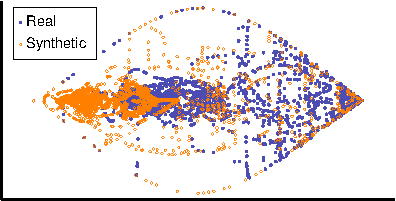
\includegraphics[scale=\scale]{Images/pca-mf.pdf}}
    \hfill
    \subfloat[Least Forgiving]{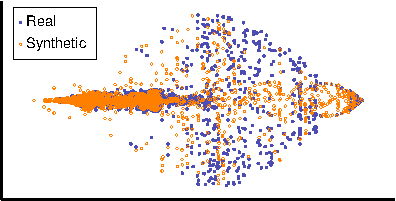
\includegraphics[scale=\scale]{Images/pca-lf.pdf}}
    \caption{PCA output of real vs. synthetic mixed data based on FL strategy.}
    \label{fig:pca-decentralized}
\end{figure}



